\documentclass[12pt, a4paper]{article}
\usepackage{enumerate}
\usepackage{graphicx,subfigure}
\usepackage{amsmath,amsthm,amsfonts,amssymb,bm}
%\usepackage{txfonts}
\usepackage[BoldFont,SlantFont,CJKchecksingle]{xeCJK}
%\setCJKmainfont[BoldFont=SimHei]{SimSun}
%\setCJKmonofont{SimSun}
%\setmonofont{Consolas}
\usepackage{longtable,multirow}
\usepackage{color,xcolor}
%\usepackage{courier}
\usepackage{ifthen}
\usepackage{calc}
\usepackage{ifpdf}
\usepackage{titling}
\usepackage{listings}
\usepackage{fancyhdr}
\usepackage{booktabs}
\usepackage{ulem}
\usepackage{lastpage}
\usepackage{lipsum}
\usepackage{mathtools,framed,graphicx,xcolor}
\usepackage{titlesec}
\usepackage{makecell}
\usepackage{tabularx}
\usepackage{fancyvrb}
\usepackage{enumitem}
\usepackage{tabto}
\usepackage{ulem}
\usepackage[colorlinks,linkcolor=blue,urlcolor=blue]{hyperref}
\usepackage{ifxetex,ifluatex}
\usepackage{caption}

\XeTeXlinebreaklocale "zh"
\XeTeXlinebreakskip = 0pt plus 1pt minus 0.1pt

\usepackage[T1]{fontenc}
\usepackage{indentfirst}
\setlength{\parindent}{2em}
\renewcommand{\baselinestretch}{1.3}

%% 页边距
\setlength{\textwidth}{\paperwidth}
\setlength{\textheight}{\paperheight}
\setlength\marginparwidth{0cm}
\setlength\marginparsep{0cm}
\setlength{\oddsidemargin}{0cm}
\setlength{\evensidemargin}{\oddsidemargin}
\setlength{\voffset}{-0.5cm-20pt}
\addtolength{\textwidth}{-2in}
\setlength{\topskip}{0pt}
\setlength{\skip\footins}{15pt}
\setlength{\topmargin}{0cm}
\setlength{\footskip}{1.5cm}
\setlength{\headsep}{0.5cm}
\addtolength{\textheight}{-2in-1.5cm+0.5cm+20pt}

\title{LemonPlus 用户手册}
\author{浮尘ii*}
\date{}

\begin{document}
\maketitle
\tableofcontents

\newpage

\section{项目介绍}
LemonPlus 项目 fork 自 \href{https://github.com/zhipeng-jia/project-lemon}{Lemon},使用 Qt5 进行了重构,新增了适合新时代 OI 的功能,移除了一些不稳定的、过时的功能。

LemonPlus 最重要的改动在于对捆绑测试 (Subtask) 的支持以及对交互式试题的支持,同时增加了可选的子文件夹、适配高分屏、自定义最大重测次数、单题评测等功能。

同时 LemonPlus 是完全兼容 Lemon 的,也就是说使用 Lemon 创建的比赛不用更改就可以使用 LemonPlus 打开并进行评测。

LemonPlus 项目的仓库地址为 \url{https://github.com/Dust1404/Project_LemonPlus},Linux 用户可以尝试使用 \href{https://github.com/iotang}{iotang} 维护的 \href{https://github.com/iotang/Project_LemonPt}{LemonPt},LemonPt 项目是 fork 自 LemonPlus 项目并针对 Linux 系统进行了二次开发。

本篇用户手册是仿照 Lemon 的用户手册进行编写的。

\begin{center}

\includegraphics{pic/icon.png}
\end{center}

\newpage

\section{安装}

LemonPlus 在上文中提及的\href{https://github.com/Dust1404/Project_LemonPlus}{仓库地址}不仅用来存储源代码,也用来实时发布软件最新版本。

\subsection{Windows 平台}
打开项目仓库地址,下载 \texttt{Release} 文件夹中的 \href{https://raw.githubusercontent.com/Dust1404/Project_LemonPlus/master/Release/windows_release.7z}{windows\_release.7z}。

或者在 \href{https://github.com/Dust1404/Project_LemonPlus/releases}{Release} 中下载 \texttt{lemonPlus-windows\_release.7z},注意,此处的版本可能较老。

下载完压缩包后,解压缩至某一文件夹,双击 \texttt{lemon.exe} 即可运行。

\subsection{Linux 平台}\label{linux install}
Linux 平台下的安装大同小异,这里以 Ubuntu 平台为例。

首先安装一些工具,打开终端输入:

\begin{lstlisting}[language=bash,frame=shadowbox,basicstyle=\ttfamily]
sudo apt install g++ gcc qt5-default make
\end{lstlisting}

然后可以使用 git 或者在网页中下载源代码,这里不赘述下载过程。

下载好后,目录切换至 LemonPlus 目录内,依次运行:

\begin{lstlisting}[language=bash,frame=shadowbox,basicstyle=\ttfamily]
gcc watcher_unix.c -o watcher_unix -O2
gcc realjudge.c -o realjudge_linux -O2
qmake lemon.pro
make
\end{lstlisting}

注意,\texttt{watcher\_unix} 和 \texttt{realjudge} 两个文件在不同计算机上应重新编译,否则评测时可能会出现无法运行程序的错误。

这时目录下已经编译出了可执行文件,使用 \texttt{./lemon} 就可以运行 lemonPlus。

\newpage

\section{配置}

LemonPlus 第一次运行时会自动弹出添加编译器的向导,具体的说明请看编译器配置一节。

\subsection{常规配置}
LemonPlus 运行后会弹出打开或新建比赛的对话框,先选择取消关闭这个对话框,然后再工具菜单中选择“选项”,就能看到下图所示的对话框:

\begin{center}
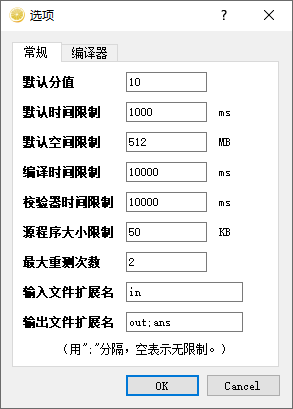
\includegraphics[scale=0.7]{pic/generalsettings.png}
\end{center}

各个设置意义如下:

\begin{description}
\item[默认分值] 新建一个测试点时的默认分值,可以设置的最大值为 100。
\item[默认时间限制] 新建一个测试点默认的时间限制,可以设置的最大值为 $6 \times 10^5$ ms,即 10 分钟。
\item[默认空间限制] 新建一个测试点时默认的空间限制,可以设置的最大值为 1024 MB。
\item[编译时间限制] 测试时允许编译器运行的最长时间,可以设置的最大值为 $6 \times 10^5$ ms,即 10 分钟。
\item[检验器时间限制] 对于使用自定义校验器的试题,测试时允许校验器运行的最长时间,可以设置的最大值为 $6 \times 10^5$ ms,即 10 分钟。
\item[源程序大小限制] 测试时可以接受的最大源程序大小,可以设置的最大值为 10240 KB,即 10 MB。
\item[最大重测次数] 当测试某测试点时程序运行时间不超过时间限制的 1.1 倍或超时不超过 100ms 时,LemonPlus 会对该测试点进行重测。限制最多重测几次,可以设置的最大值为 10。
\item[输入、输出文件扩展名]  在自动添加试题时扫描的输入和输出文件的扩展名。如果有多个请用 \texttt{';'} 隔开。每种扩展名中只能包含英文字母和数字,Linux 平台下大小写是敏感的。注意这里的扩展名只供添加测试点时软件搜索文件使用,测试时并不会检查。
\end{description}

\subsection{编译器配置}
点击上方的 “编译器” 选项卡就能进入编译器的配置。

\begin{center}
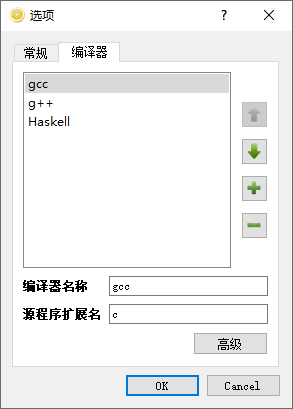
\includegraphics[scale=0.7]{pic/compilersettings.png}
\end{center}

按右边的加号就会出现添加编译器的向导,第一步是选择使用预置的编译器配置还是手动配置新的编译器。一般来说,用预置的配置就能够满足大多数需求,第一步只要在需要配置的编译器前打钩,进入下一步后就能看到选择路径的界面。

\begin{center}
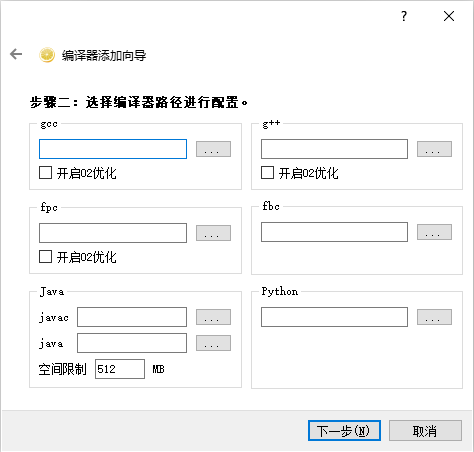
\includegraphics[scale=0.6]{pic/addcompiler.png}
\end{center}

\texttt{gcc}、\texttt{g++} 和 \texttt{fpc} 的 O2 优化是一种编译器执行的代码优化,可以一定程度提高程序运行效率。

\texttt{Java} 的内存限制是由 Java 虚拟机限制的,你可以选择不限制内存。

最后一步会让你确认编译器路径是否设置正确。

除了使用内置的六种编译器配置,你也可以选择手动配置新的编译器。

\begin{center}
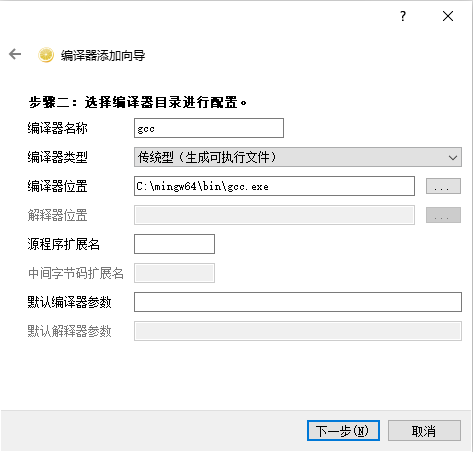
\includegraphics[scale=0.6]{pic/addcompiler2.png}
\end{center}

\begin{description}
\item[编译器名称] 编译器在列表中显示的名称。
\item[编译器类型] 总共有三种类型可选,括号里给出了相关解释。\texttt{C++}、\texttt{Java} 和 \texttt{Python} 分别是三种类型的典型代表。
\item[编译器位置] 如果编译器的类型是传统型或需要编译的解释型,这里就要选择编译器的位置。对于传统型,编译器会将源代码直接转换成机器代码,而解释型的编译器会生成中间字节码。
\item[解释器位置] 如果编译器的类型是解释型,就要选择解释器的位置。解释器用于执行中间字节码或直接解释执行源代码。
\item[源程序扩展名] 用于判断哪些扩展名的源程序使用这个编译器编译,如果有多个扩展名请用 \texttt{';'} 隔开。
\item[中间字节码扩展名] 解释型编译器生成的中间字节码的扩展名,例如 \texttt{Java} 的中间字节码扩展名为 \texttt{.class}。
\item[默认编译器参数] 编译时传递给编译器的参数,其中用 \texttt{\%s} 表示不带扩展名的源程序文件名,\texttt{\%s.*} 表示带扩展名的源程序文件名。例如 \texttt{gcc} 的编译参数为
\begin{lstlisting}[frame=shadowbox,basicstyle=\ttfamily]
-o %s %s.*
\end{lstlisting}
\item[默认解释器参数] 运行解释器时传递的参数,表示的方法同编译器参数。
\end{description}

向导完成后,我们再回到编译器管理的选项卡。

如果要删除当前选择编译器,可以按右边的减号。

右边的上下箭头是用来调整编译器优先级的。

编译器的优先级是指:如果选手对于同一道题提交了多种扩展名的源程序,排在前面的编译器会被先考虑,同时在源程序扩展名中设置排在前面的扩展名会被先考虑。

注意到下面有高级按钮,可以修改已有编译器的配置。

\begin{center}
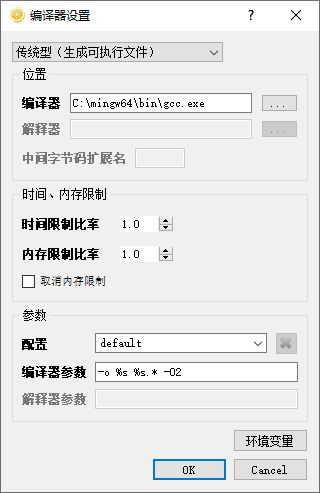
\includegraphics[scale=0.7]{pic/compilersettings2.png}
\end{center}	

由于不同语言执行效率有差异,因此可以放宽特定语言的时间限制或空间限制,也就是将时间限制或空间限制乘上一个实数,对于空间限制,也可以选择直接取消。

每个编译器都可以有多个配置,不同配置的编译参数或解释器运行参数不同,一般用于选择不同的优化开关。

点击环境变量按钮可以设置编译器和程序运行时额外设置的环境变量,一般用于保证运行所需的动态链接库文件能被找到。

\newpage

\section{新建比赛}

运行软件后会弹出 “欢迎” 对话框,可以选择打开已有的比赛或者新建比赛。如果关闭了这个对话框,也可以在文件菜单中选择打开或新建比赛。

新建比赛的对话框如下图所示:

\begin{center}
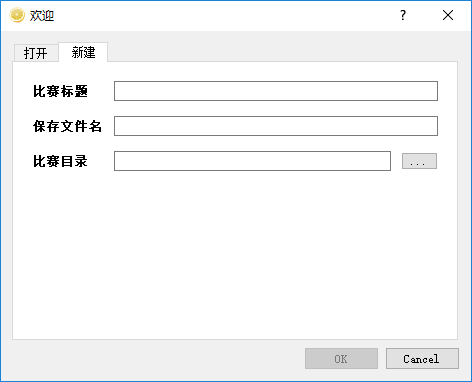
\includegraphics[scale=0.7]{pic/newcontest.png}
\end{center}

\begin{description}
\item[比赛标题] 用来显示在软件标题栏上的比赛标题。
\item[保存文件名] 保存比赛文件使用的文件名,这里输入的不需要附带扩展名。
\item[比赛目录] 比赛相关文件的存储目录。  
\end{description}

点击确定后,软件会在制定的比赛目录下创建 \texttt{data} 和 \texttt{source} 目录,同时还有一个扩展名为 \texttt{cdf} 的文件名用来保存试题、选手信息。

其中 \texttt{data} 下用来存放试题的数据、自定义的校验器、交互题的交互库、接口实现等文件,\texttt{source} 目录下存放每个选手的源程序或答案文件。

\texttt{source} 目录下的每个文件夹代表一位选手,文件夹的名称为选手的名称。每位选手的文件夹是否需要对每个题目建立子文件夹可以在题目页面设置,见以下内容。

你可以使用文件菜单栏中的 “打开当前比赛目录” 来打开当前比赛的目录。

\subsection{添加新试题}

建立好比赛后,在左边按鼠标右键就可以添加新的试题。然后在右边设置试题相关的信息。

\begin{center}
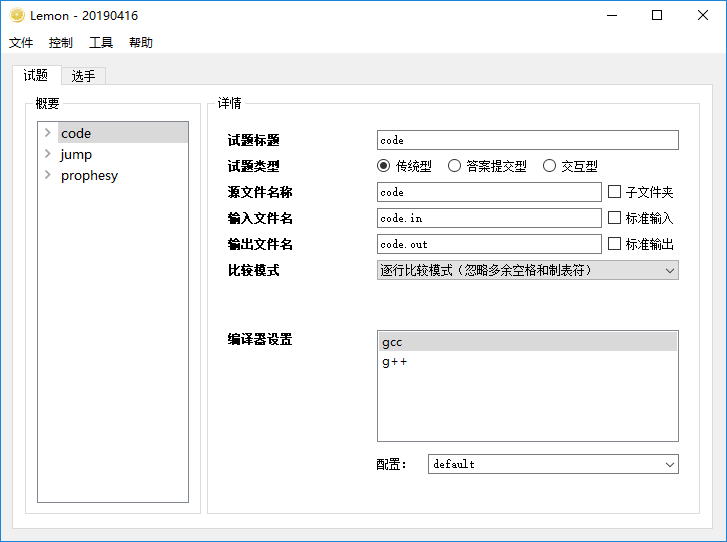
\includegraphics[scale=0.7]{pic/editproblem.png}
\end{center}

\begin{description}
\item[试题标题] 试题在列表中显示的名称。
\item[试题类型] 试题的类型,目前可用的选择有传统型、答案提交型和交互型,其中交互型只支持 NOI 风格的 C++ 语言交互。
\item[源文件名称] 源程序的文件名,注意不要带扩展名。
\item[子文件夹] 若勾选,选手目录中需要为每个题单独建一个以源文件名称(提交答案型为试题名称)命名的文件夹,将源程序放在文件夹内;否则只需要将源程序放在选手目录下即可。
\item[输入、输出文件名] 选手程序使用的输入输出文件名。
\item[标准输入、输出] 若勾选,则选手程序会从标准输入读入数据(或向标准输出输出数据),不使用文件 IO。
\item[比较模式] 比较选手输出和标准输出的方式,目前有五种方式:逐行比较模式、忽略多余空格和制表符的逐行比较模式(默认)、外部工具模式、实数比较模式(不推荐)和自定义校验器。

逐行比较模式会一行一行比较选手的输出和标准输出是否相同,不同系统平台的换行符不同不会产生影响。

逐行比较模式中也可以选择忽略多余的空格和制表符。

外部工具模式会调用 Linux 下的 \texttt{diff} 命令进行比较,Windows 下也可以使用,但是要将 \texttt{diff.exe} 放在和 \texttt{lemon.exe} 相同的目录下,Release 压缩包中已经包含。

实数比较模式会注意读取选手输出和标准输出中的每一个实数,分别比较误差是否在允许范围内,由于可能有 \texttt{nan} 和 \texttt{inf} 的存在,不推荐使用此方式,可以使用自定义校验器实现实数比较。

自定义校验器 需要选择一个可执行文件作为校验器,具体的说明请参见下一个章节。
\item[编译器配置] 为每个编译器选择配置,也就是选择相应的编译参数,默认会选择 \texttt{default} 配置。
\item[选手答案文件扩展名] 对于提交答案题,选手提交的答案文件中,每个文件会和输入文件中去除扩展名后文件名一样的那个配对,这里可以设置选手提交的答案文件的扩展名,默认为 \texttt{out}。
\item[交互库路径] 对于交互型试题,使用的交互库路径,通常为 \texttt{.h} 或 \texttt{.hpp} 文件。
\item[交互库名称] 指选手需要引用的头文件名称。
\item[接口实现(grader)路径] 主要是不太会翻译这个东西,一般为一个 \texttt{grader.cpp} 文件实现交互库中的接口。   
\end{description}

\subsection{自定义校验器说明}
自定义校验器需要为一个可执行文件,评测软件通过将一些参数传给校验器,使得校验器获得输出、输出文件等信息,然后将得分的结果写入指定文件中。

评测软件会向校验器传入六个参数,按照顺序分别表示标准输入文件、选手输出文件、标准输入文件、本测试点满分、分数输出文件、额外信息文件。

其中分数输出文件必须创建,需要向其中写入一个非负整数表示得分。

额外信息文件可以不创建,如果创建了可以写入任何信息,这些信息会显示在结果中。

\subsubsection{校验器实例}
实现一个校验器实现误差为 $10^{-4}$ 的实数比较。

\newpage

\begin{lstlisting}[language={C++},numbers=left,frame=shadowbox,showspaces=false,showstringspaces=false
	rulesepcolor=\color{red!20!green!20!blue!20},
	keywordstyle=\color{blue!70!black},
	commentstyle=\color{blue!90!},
	basicstyle=\ttfamily]
#include <stdio.h>
#include <math.h>

int main(int argc, char **argv)
{
	FILE *fin = fopen(argv[1], "r");
	FILE *fout = fopen(argv[2], "r");
	FILE *ans = fopen(argv[3], "r");

	FILE *score = fopen(argv[5], "w");
	FILE *msg = fopen(argv[6], "w");

	double yourAnswer, stdAnswer;

	fscanf(fout, "%lf", &yourAnswer);
	fscanf(ans, "%lf", &stdAnswer);

	if (fabs(yourAnswer - stdAnswer) < 1e-4)
	{
		fprintf(score, "%s\n", argv[4]);
		fprintf(msg, "Correct Answer\n");
	}
	else
	{
		fprintf(score, "0\n");
		fprintf(msg, "Wrong Answer\n");
	}

	fclose(fin);
	fclose(fout);
	fclose(ans);
	fclose(score);
	fclose(msg);

	return 0;
}
\end{lstlisting}

\subsubsection{使用 testlib}
testlib 的使用说明可以在 \href{https://oi-wiki.org/intro/testlib/}{OI Wiki} 上见到,在此不再赘述。

Lemon 所需的修改版 testlib 可以在\href{https://paste.ubuntu.com/p/JsTspHHnmB/}{这里}获取到,感谢 matthew99。

注册 checker 只需要执行一句 \texttt{registerLemonChecker()} 即可。

使用 testlib 编写的上节中的自定义校验器如下:

\begin{lstlisting}[language={C++},numbers=left,frame=shadowbox,showspaces=false,showstringspaces=false
	rulesepcolor=\color{red!20!green!20!blue!20},
	keywordstyle=\color{blue!70!black},
	commentstyle=\color{blue!90!},
	basicstyle=\ttfamily]
#include <cmath>
#include "testlib.h"

int main(int argc, char **argv)
{
	registerTestlibCmd(argc, argv);

	double pans = ouf.readDouble();
	double jans = ans.readDouble();

	if (abs(pans - jans) < 1e-4)
		quitf(_ok, "Correct Answer\n");
	else
		quitf(_wa, "Wrong Answer\n");
	
	return 0;
}
\end{lstlisting}

\subsection{关于非传统型试题}

本节介绍了非传统型试题与传统题的区别以及测评逻辑。

\subsubsection{提交答案型试题}

提交答案型试题中,选手不需要提交源程序,只需要提交答案文件。

所以测评中,不需要进行源程序的编译、运行,直接对答案进行判断即可。

选手提交的答案文件名应与测试点配置中的输入文件相同(不包括扩展名),扩展名与题目配置的答案文件扩展名相同,软件将对选手提交的文件与测试点配置的答案文件以配置的比较模式进行比较。

\subsubsection{交互型试题}

只支持 NOI 风格的 C++ 语言交互。

编译时将交互库拷贝至编译临时目录下并命名为交互库名称,将接口实现文件拷贝至目录下,进行双文件编译。

对于交互库全部写在一个库文件中的题目(不推荐,选手可能会通过扫内存等方式获得信息),可以创建一个空的接口实现文件 \texttt{grader.cpp} 完成配置,不影响编译。

\subsection{添加新测试点}

在左边选中一道试题后,右键鼠标出现菜单,选择“添加测试点”即可添加一个新的测试点,右边会变成测试点设置界面。

在输入文件名和输出文件名中输入内容后,点击“添加”按钮即可添加一组测试数据。这里的输入输出文件必须在 \texttt{data} 目录下,并且只要输入 \texttt{data} 目录内的相对路径即可,如下图所示:

\begin{center}
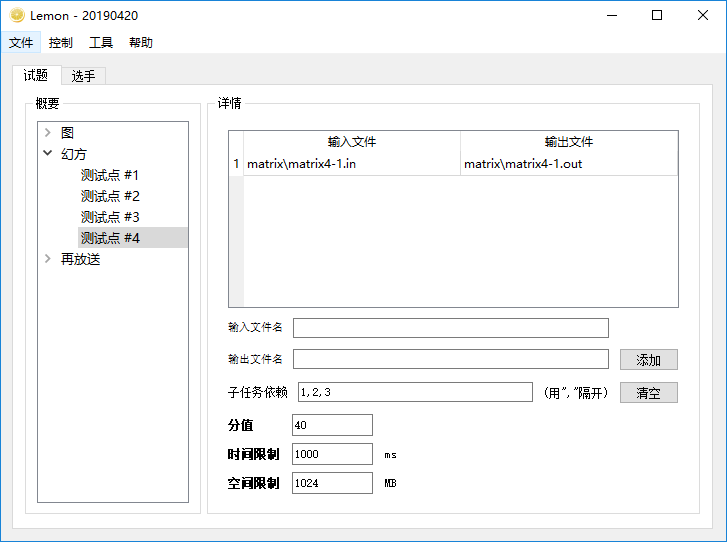
\includegraphics[scale=0.7]{pic/edittestcase.png}
\end{center}

一个测试点可以包含多组输入输出,最终一个测试点的得分为该测试点包含的所有测试数据中最低的得分。

同时支持子任务依赖,对于测试点 $i$,请保证输入的子任务编号在 $[1, i - 1]$ 之间,多个依赖项之间用 \texttt{,} 隔开。子任务依赖的意思是该测试点得分百分比不超过这些测试点中任意一个的得分百分比(即该测试点得分会对所有依赖的测试点的得分百分比乘该测试点总分取最小值)。

如果要编辑输入输出文件名,直接在表格相应位置双击即可修改。

选中一行或多行后按 \texttt{Delete} 键,即可删除对应的输入输出文件。

在下面可以设置本测试点的分值、时间限制和空间限制。可以设置的最大分值为 100,最大时间限制为 $6 \times 10^5$ ms(10 分钟),最大空间限制为 1024 MB。

\subsection{批量添加测试点}

在左边选中一道试题后右键鼠标出现菜单,选择 “添加多组测试点...” 后会弹出一个向导,用来批量添加测试点。

向导的第一步是设置每个测试点的分值、时间限制和空间限制,当然也可以添加完成后在编辑页面更改。

第二步是设置如何匹配输入、输出文件名,这里需要会使用简单的正则表达式。

输入、输出文件格式中可以使用 \texttt{<1>},\texttt{<2>},...,\texttt{<9>} 来表示一个正则表达式,然后在下面按右边的加号可以先见这样一个参数并指定参数代表的正则表达式。需要注意的是在输入文件格式和输出文件格式中,每个参数只能出现一次。

对于所有参数匹配内容都相同的文件,会作为一组输入输出。

对于打钩的参数匹配内容都相同的输入输出,会放在同一个测试点中。

以一道捆绑测试的试题为例,在 \texttt{data} 下的 \texttt{wander} 文件夹里,有 \texttt{wander(x)-(y).in/out} 文件代表第 $x$ 个子任务的第 $y$ 个测试点的输入输出文件,那么匹配参数可以按照下图:

\begin{center}
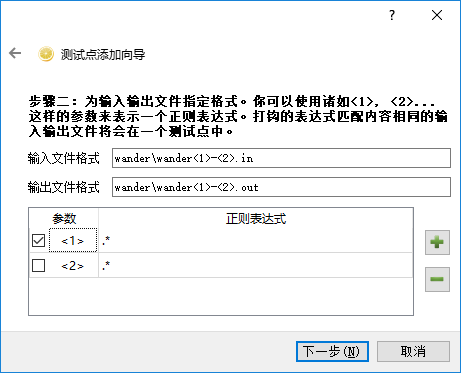
\includegraphics[scale=0.6]{pic/addtestcases.png}
\end{center}

注意:Windows 下文件夹分隔符为 \texttt{\textbackslash},Linux 下文件夹分隔符为 \texttt{/}。

最后一步是预览结果,如果发现结果和预期的不同可以回到上一步修改参数。

\subsection{自动添加试题}
为了简化试题、测试数据的添加过程,Lemon 作者设计了自动添加试题功能。对于一道试题,如果希望能够自动添加,请在 \texttt{data} 目录中为这个试题创建一个文件夹,将相对应的数据文件放入文件夹中。然后再控制菜单中选择 “自动添加试题”,会出现一个对话框,给出找到的试题。

可以设置每道试题所有测试点的总分值、所有测试点的时间限制和空间限制,确定后就会自动添加相应的试题。

自动添加的试题默认作为传统型试题,添加后的试题标题和源程序名称都是对应试题的文件夹名称,输入输出文件分别再加上扩展名 \texttt{in} 和 \texttt{out}。

数据文件的匹配方法是:根据设置中设定的输入输出文件扩展名,选出相应的文件,如果在设置中输入或输出文件扩展名为空,会自动将输入文件扩展名设置为 \texttt{in},输出文件扩展名设置为 \texttt{out;ans}。

然后对于除扩展名外文件名相同的文件会被作为一组输入输出,并为这一组输入输出创建一个测试点,注意文件名的大小写是敏感的。

用 “自动添加试题” 功能添加的试题,每个测试点只会有一组输入输出。

每个测试点的分值会用设置的总分除以测试点个数,由于分值只能是整数,没法除尽时会向下取整。

请尽量保证输入输出文件能够按上述方法唯一配对,否则产生的结果不可预料。

其中可以设置的试题总分值最大为 $10^5$,时间限制最大为 $6 \times 10^5$ ms(10 分钟),空间限制最大为 1024MB。

\section{开始测试}
点击“选手”选项卡,按下面的“刷新”按钮后,就会根据 \texttt{source} 目录下的文件夹添加列表中不存在的选手,并从列表中删除已经从 \texttt{source} 目录中删除的选手。

然后单击 “测试全部” 按钮就能开始测试。注意选手提交的程序名在 Linux 下是大小写敏感的。

单击 “单题测试” 按钮可以对所有选手的某一题进行重测。

选中单个或多个选手后按 “测试” 按钮可以仅测试选中的部分选手,按 \texttt{Delete} 键或右键点击删除可以删除选中的选手。

测试完成后通过在表头上单击可以按照相应的项目排序。

双击一名选手可以查看详细的测试结果并对该选手的某一题进行重测。

测试过程中会有 Subtask Skip,即对于一个测试点如果已经确定该测试点会得 0 分,则跳过改测试点剩下的所有数据,可以大大减少捆绑测试的题目的测试时间。

\section{导出成绩}
在 “控制” 菜单中选择 “导出成绩” 可以将结果导出成 HTML 文档或表格文件。

推荐使用 HTML 格式,可以导出完整的结果信息,导出成表格的话只能限制选手每道题的得分和总分。

表格有两种格式可以选择:csv 格式和 xls 格式(仅 Windows 可用并需要安装 Excel)。

csv 格式是逗号分隔符,多数表格编辑软件都能查看。xls 格式的导出需要利用 ActiveX 调用 Excel,写入速度非常慢,除非特别需要,否则不推荐使用。

\section{常见问题及回答}
在使用中出现任何问题,可以在 \href{https://github.com/Dust1404/Project_LemonPlus}{Github 仓库}中的 Issue 提出。

此节内容长期更新,更多问题欢迎提出。

\subsection{测评时使用更多栈空间}
Windows 平台下可以在 \texttt{g++} 编译时添加 \texttt{-Wl,--stack=1073741824} 命令来开启 1024MB 栈空间。

Linux 平台下(以 Ubuntu 为例)可以在终端中先输入如下命令:
\begin{lstlisting}[language=bash,frame=shadowbox,basicstyle=\ttfamily]
ulimit -s unlimited
\end{lstlisting}

然后再用此终端打开 Lemon,或者可以使用 \href{https://github.com/iotang}{iotang} 维护的 \href{https://github.com/iotang/Project_LemonPt}{LemonPt}。

\subsection{Linux 下无法运行程序,临时目录下出现乱码}
这是安装时没有在本机编译 \texttt{watcher\_unix.c} 造成的,建议按照 \hyperref[linux install]{安装方法} 重新安装。

\end{document}